% NIH Grant Proposal for the Specific Aims and Research Plan Sections
%----------------------------------------------------------------------------------------
%	PACKAGES AND OTHER DOCUMENT CONFIGURATIONS
%----------------------------------------------------------------------------------------

\documentclass[11pt,notitlepage]{article}

% A note on fonts: As of 2013, NIH allows Georgia, Arial, Helvetica, and Palatino Linotype. LaTeX doesn't have Georgia or Arial built in; you can try to come up with your own solution if you wish to use those fonts. Here, Palatino & Helvetica are available, leave the font you want to use uncommented while commenting out the other one.

\usepackage[super]{natbib}
\usepackage{palatino} % Palatino font
%\usepackage{helvet} % Helvetica font
\renewcommand*\familydefault{\sfdefault} % Use the sans serif version of the font
\usepackage[T1]{fontenc}
\linespread{1.05} % A little extra line spread is better for the Palatino font
\usepackage{hyperref} % to allow hyperlinks to websites on the internet
\usepackage[hypcap]{caption} % to point to the top of the image
\usepackage{lipsum} % Used for inserting dummy 'Lorem ipsum' text into the template
\usepackage{amsfonts, amsmath, amsthm, amssymb} % For math fonts, symbols and environments
\usepackage{graphicx} % Required for including images
\usepackage{booktabs} % Top and bottom rules for tables
\usepackage{wrapfig} % Allows in-line images
%\usepackage[labelfont=\small]{caption} % Make figure numbering in captions bold
\usepackage[top=0.6in,bottom=0.6in,left=0.6in,right=0.6in]{geometry} % Reduce the size of the margin

\usepackage{booktabs}
\usepackage{graphicx}
\usepackage[table,xcdraw]{xcolor}
\pagestyle{empty} % Remove page numbers
%\let\oldtabular\tabular 
%\renewcommand{\tabular}{\large\oldtabular}

\hyphenation{ionto-pho-re-tic iso-tro-pic fortran} % Specifies custom hyphenation points for words or words that shouldn't be hyphenated at all

  % to reduce white space between SECTIONS
\usepackage[compact]{titlesec}
%\titlespacing{\part}{-200pt}{-50pt}{-40pt}
%\titlespacing{\subsection}{0pt}{*0}{*0}
%\titlespacing{\subsubsection}{-2pt}{*0}{*0}
%\titlespacing{\subparagraph}{-5pt}{*0}{*0}
%\titlespacing*{\subparagraph} {\parindent}{1ex plus 1ex minus .2ex}{0.5em}

  
  % to reduce white space between PARAGRAPHS
%\setlength{\parskip}{-2pt}
% \setlength{\parsep}{-2pt}

  % additional parameters
%\setlength{\headsep}{0pt}
%\setlength{\topskip}{0pt}
%\setlength{\topmargin}{0pt}
%\setlength{\topsep}{0pt}
%\setlength{\partopsep}{-2pt}
%\setlength{\parindent}{1cm}

% to reduce white space around figures
% \setlength{\textfloatsep}{0pt plus 0pt minus 0pt}

\begin{document}
\part*{Specific Aims}
National health databases and electronic health records (EHR) are inherently clustered by procedure, provider, service, institution and geography. Their rich spatial and temporal organization is most realistically captured in multilevel hierarchical statistical models, but efficient model fit and computational implementation are still difficult. We propose to further develop Stan, a novel, probabilistic programming language, to make advanced hierarchical modeling more readily accessible to data scientists for outcome and health services research. 

\paragraph*{Flexibility and robustness of hierarchical modeling could transform EHR based outcomes research.} We consider surgery as an illustrative example. Patients in the same hospital undergoing the same surgical intervention by the same team will show similar clinical trajectories and responses. Typically we are interested to investigate differences in therapeutic effects or to predict poor outcomes to prevent them. (1) By estimating individual effects for each provider or procedure, random effects can help to control for potentially confounding differences in quality of care by different teams. (2) Spatial clustering of adherence behavior , e.g by different services, can be represented by multilevel modeling. (3) Especially in subgroups with sparse data, partial pooling can improve parameter estimates; for example prediction of poor health outcomes can be improved by exploiting the implied correlations using information from different but related subsets. Failure to account for the highly structured and correlated nature of health care delivery may lead to incorrect statistical inferences.

\paragraph*{Hierarchical modeling and related diagnostics should be readily accessible to clinical data scientists.} At present, it still takes a computationally sophisticated statisticians to write complex hierarchical models, transform the data or parameters to facilitate model convergence and index the group indicators in a multilevel hierarchical model error free. We lack intuitive diagnostic, visual and exploratory tools to address convergence and model fit. Model convergence diagnostics and troubleshooting algorithms are still underdeveloped. 

\paragraph*{Classical approaches and software packages often lack flexibility for multilevel hierarchical modeling.} Available algorithms are slow to converge even on advanced workstations, if they converge at all. Stan, our flexible general-purpose modeling language facilitated much more widespread multilevel modeling statistics in biostatistics, epidemiology, public health and political science and pharmacokinetic modeling. Stan's novel Hamiltonian Monte Carlo algorithm converges faster by orders of magnitude and is ideally suited to fit even advanced and unorthodox statistical models. Stan's development was funded through the NSF; therefore Stan and its algorithms are open source; they are implemented on multiple platforms (Python, Julia, R/Rstudio). 

\paragraph*{Robust, efficient, expressive and accessible software promotes Big Data outcomes research.} We propose to further simplify complex multilevel model building for clinical and health services research by developing additional and more user friendly open source software packages around Stan, incorporating interactive, intuitive visual and novel statistical tools to facilitate principled model optimization and checking. 

\subparagraph{Specific aims}
\paragraph*{Aim 1:} To develop simple and user-friendly software packages around Stan in the open-source statistical computing environment R/Rstudio in collaboration with applied clinical data scientists and biostatisticians. To make complex hierarchical modeling of EMR computationally efficient and readily accessible to average clinical data scientists with a simple standardized function call to a representative class of multilevel models.

\paragraph*{Aim 2:} To develop an interactive diagnostic software package to analyze and visually explore the convergence and output of complex hierarchical models and to develop novel principled diagnostic algorithms and utilities to diagnose and troubleshoot non-convergence, detect multidimensional co-linearity and accelerate computational implementation of advance hierarchical models.

\paragraph*{Aim 3:} To explicate, document and disseminate complex hierarchical modeling and its advanced computational implementation in collaboration with the clinical Big Data science community with hands on workshops, e-books, online tutorials and electronic resources. To solicit the Big Data community feedback, engage new software developers and to incorporate corrections into our software through online user and developer groups.

\part*{Research Strategy}

\part*{Significance}

\section*{The nested structure of health care delivery and electronic health data}
Clinical data scientists are faced with an abundance of useful electronic health data, but limitations of existing statistical inference tools constrain the scientific hypotheses they can be explore and evaluate. Electronic health related data sets are not only growing exponentially in number of units of observations or variables observed, but this growth implies increasingly complex interactions and correlations. 

\subsection*{National Anesthesia Clinical Outcomes Registry is an example of hierarchically structured health data}
We will illustrate the clustered, nested data structure of contemporary health care delivery and electronic health data capture with the example of the National Anesthesia Clinical Outcomes Registry (NACOR), maintained by the Anesthesia Quality Institute and funded by the American Society of Anesthesiologists. 

\subsection*{Perioperative health care delivery and data capture are nested and clustered.}
Anesthesia is an illustrative case of the how health care is increasingly electronically documented, facilitating the continuous registration of multiple simultaneous physiological   data and therapeutic interventions during critical interventions. To support billing, this electronically captured data set is jointed with surgical and anesthesia procedure codes, International Classification of Disease (ICD) codes, provider identifiers, patient perioperative risk, outcome and provider compliance assessment. Participating institutions upload this comprehensive file from their anesthesia information management systems (AIMS) directly to NACOR. NACOR contains at present over 30 million individual electronic records of anesthesia care provided; like similar databases, NACOR is growing exponentially. This data mine invites health services and outcomes research.

\subsection*{Care delivered and outcomes achieved depend on procedure, providers and patient characteristics.} For example, the particular anesthetic a given individual receives will depend on the surgical procedure the patient is undergoing and under which service, but also on the local institutional culture and indeed the individual anesthesia provider and his or her qualifications and preferences\cite{AndreaeWhite2015}; We seek to substantiate the nested structure of outcome data in health care with two examples from (1) labor analgesia and (2) spine surgery : 

(1) Anesthesiologists may feel more or less inclined or competent to offer regional anesthesia techniques; provision of epidural labor anesthesia varies widely across the nation and within an institution and is predicted by socioeconomic and racial patient characteristics \cite{Rust2004,Glance2007}.
 
(2) Bleeding during spine surgery is substantially less, if performed by a neurosurgeons versus by an orthopedic surgeon; while true on average, an individual gifted orthopedic surgeon may outperform the average neurosurgeon with regards to surgical blood loss.

\section*{Hierarchical models capture contemporary health care practice realistically}
Hierarchical modeling could transform electronic health records based outcomes research, because the evident rich spatial and temporal organization of electronic health records is most realistically captured in multilevel hierarchical statistical models. However, efficient model fit and computational implementation are still difficult.  Additional depth of data (simply more units of observation) would increase power and make our clinical data analysis easier. Rather, there is more breadth to the data: more subgroups, locations, provider or time granularity than is currently being modeled, more partial, incomplete and noisy measurements that cannot easily be incorporated into standard models, more related studies available for meta-analysis\cite{Andreae2015,Andreae2012}.

%\begin{wrapfigure}{h}{8cm} % Example figure with text wrapping around it
% \vspace{-15pt}
% 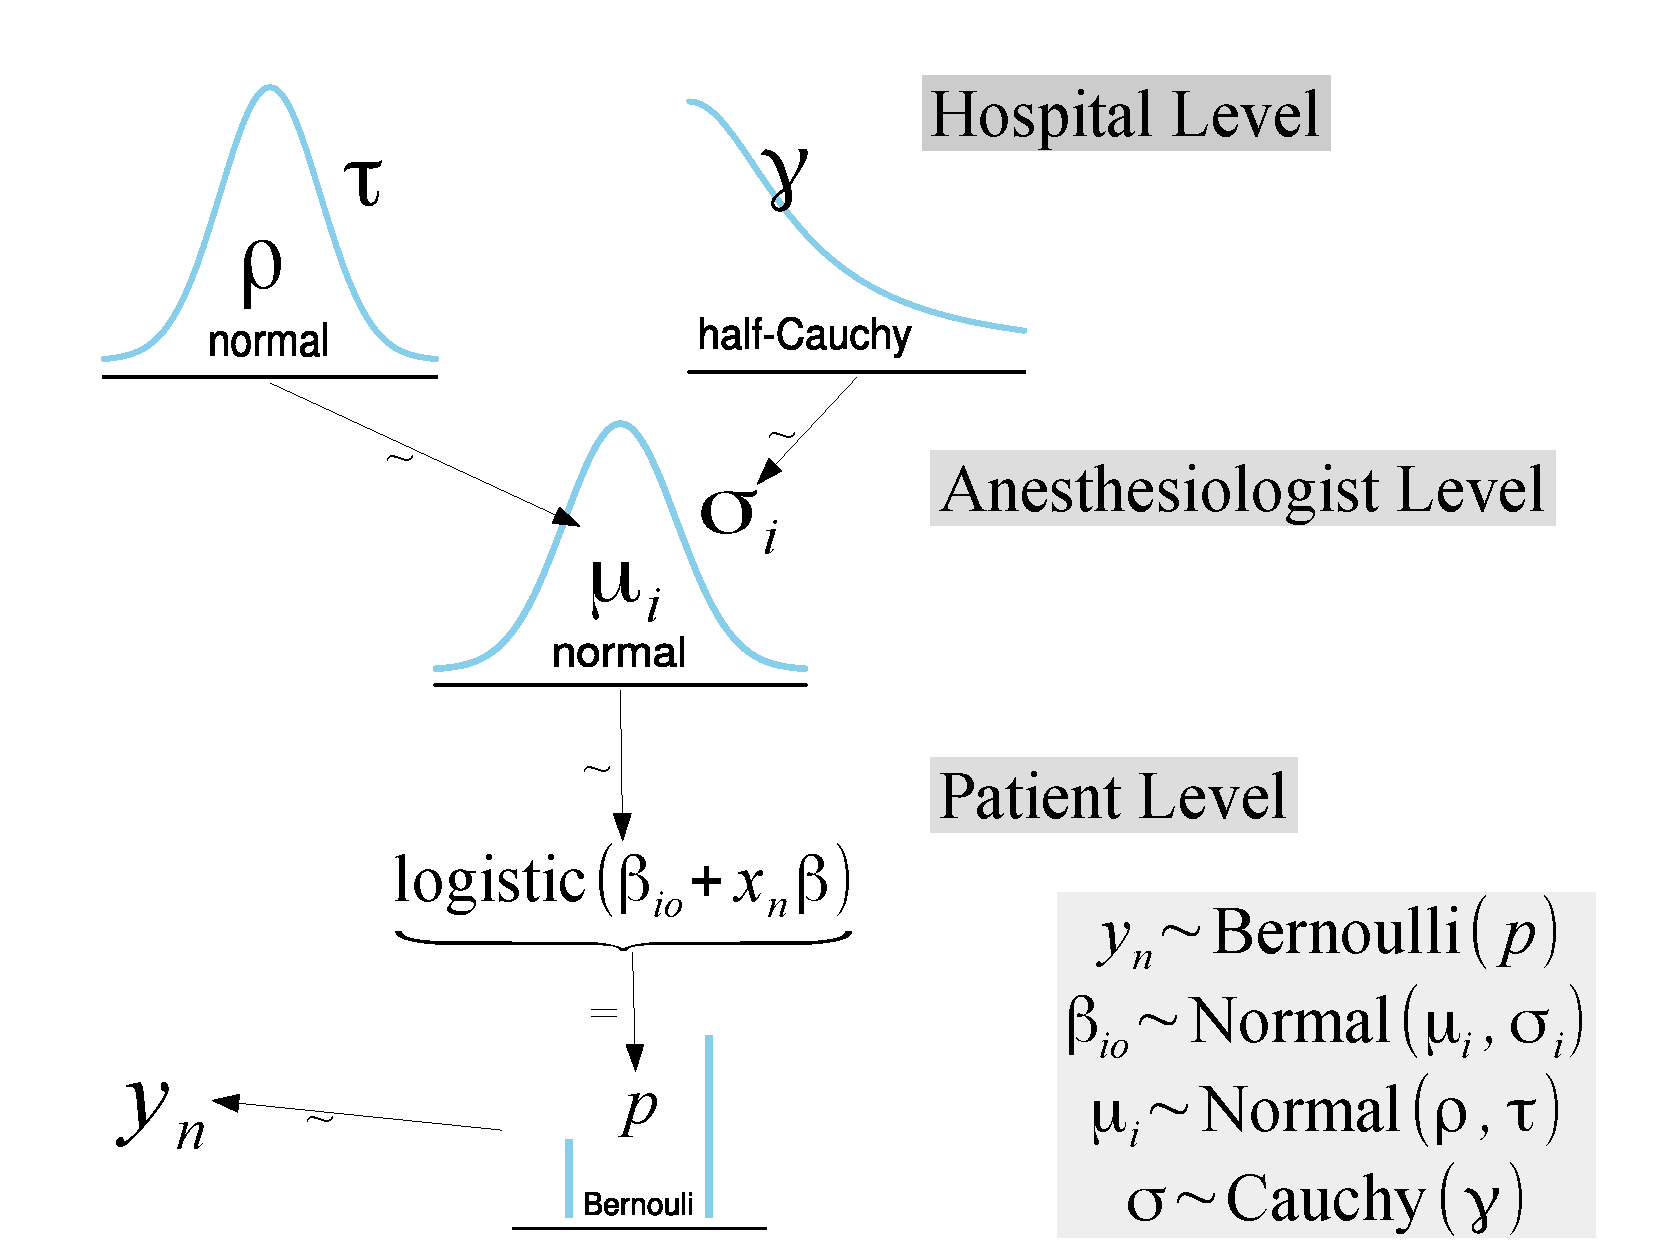
\includegraphics[scale=0.3]{Figures/DistrogramNACOR.pdf} 
%  \vspace{-20pt}
% \caption{\footnotesize Distrogram to illustrate the hierarchical structure of patient trajectories in the National Anesthesia Clinical Outcomes Registry. Outcome $y_n$ for the $n^{th}$ patient is a Boolean indicator predicted by a logistic regression. We allow the patient intercept $\beta_{oi}$ to vary according to the $i^{th}$ anesthesiology provider caring for the patient. The provider level mean $\mu_i$ and within-provider variance $\sigma_i$ are modeled to vary by hospital. $x_n$ is a vector of patient level predictors, $\beta$ is a vector of regression coefficients.}
% \vspace{-30pt}
% \label{fig:Distrogram}
%\end{wrapfigure}

\subsection*{Modeling the multifaceted correlations in EHR is reflecting actual clinical practice}
To realistically model the multifaceted correlations seen in actual clinical practice, when we fitted a regression model to investigate predictors of anesthesia quality in the NACOR database, we wanted regression coefficients to vary by provider, providers again nested by service or by hospital\cite{AndreaeWhite2015}. We needed to control for the surgical procedure type as random effect as well, with thousands of different surgical procedures performed in the NACOR population. The number of parameters to estimate grows very quickly and so do the potential interactions. Even with very large data sets, the sample size in each subgroup will shrink rapidly; estimates using least squares or maximum likelihood will become noisy and thus often become essentially useless. One solution lies in hierarchical modeling, where we estimate hyper-parameters and hyper-hyper-parameters (Figure \ref{fig:DistrogramNACOR}), to represent how lower level parameters vary across different groupings \cite{Bafumi2007}.

\subsection*{Hierarchical models provide efficient inferences with partial pooling}
Inference based on partial pooling outperforms (a) the No-pooling and (b) the complete-pooling approaches, as can be shown mathematically \cite{Efron_1975} or via cross-validation \cite{Gelman2014}.  

\begin{itemize}

\item (a) Using the No-pooling approach, we would estimate the model for each specific subset of interest separately. But this leads to far too many sub-classifications, e.g. one model for each type of surgery, thus too small samples in any given subgroup for useful inferences, if we fully explore the complexity and granularity, the richness of the EMR data. 
\item (b) Employing complete pooling or structural modeling constitutes the other extreme of the spectrum, but the implied hard constraints on the coefficients in different groups may lead to bias, negating the obvious known differences in the data, for example between patients undergoing tracheotomy versus cesarean section: we gloss over such detail and lose granularity. 
\end{itemize}

We choose the middle ground: for our richly organized NACOR data set, inference using partial pooling or hierarchical modeling is especially effective , because the estimate of each individual parameter is simultaneously informed by data from all the other patients in our cohort, improving inferences in particular for subgroups with sparse data. \cite{Gelman2009}. Effron explained this apparent paradox well to non-statisticians in the \href{http://www.nature.com/scientificamerican/journal/v236/n5/pdf/scientificamerican0577-119.pdf}{Scientific American} \cite{Efron_1977,Efron_1977a}. 

\subsection*{Meta-analysis for evidence based clinical care}

Clinicians are familiar with systematic reviews and meta-analysis\cite{Sackett1996}. Evidence synthesis (a more accurate term than meta-analysis) is a powerful tool to pool clinical trials to guide evidence based clinical care \cite{Ashby2000}. Rigorous evidence synthesis is considered the highest level of evidence to support clinical decision making \cite{Cook1997}. 

\subsubsection*{Variance in study design and outcome reporting hamper evidence synthesis}
However, studies on perioperative outcomes tend to vary in design and reported outcomes\cite{Andreae2013}, making evidence synthesis challenging with classical or frequentist statistical models\cite{Spiegelhalter2000}; not least, because often only dichotomous aggregate results are reported \cite{Roth2015CriticalCare}.  The integration of dichotomous outcomes with continuous outcomes often requires access to individual patient data, rarely available for evidence synthesis\cite{Andreae2015}. Meta-regression of effect dose dependence can explain substantial between-study variance in outcomes reported to reconcile study findings \cite{Andreae2015,Thompson2002,Abroug2011}. Different study designs can make it difficult to perform meta-analysis or meta-regression with classical statistical methods and standard systematic review software \cite{Deeks2011chapter}. Classical meta-analysis may also underestimate the between-study-variability for small numbers of trials\cite{Song2012,Cornell2014}.

\subsubsection*{The antimony of complete versus no-pooling also limits meta-analysis of perioperative outcomes}

Perioperative outcomes are often recorded at different follow intervals in different studies; some studies report repeated measures, others only a single terminal observation; This leads to the same issue of (a) complete pooling versus (b) No-pooling also in evidence synthesis \cite{Roth2015CriticalCare}.

\begin{itemize}

\item (a) Complete pooling irrespective of follow up-time.
Evidence synthesis of all effect estimates at different time points is only appropriate if the effect estimates does not depend on when it was observed. This is obviously often untenable assumption.

\item (b) No-pooling, but conducting meta-analyses at each time point: performing separate meta-analysis for each follow up time point separately, would drastically reduce sample size and hence power and precision, undermining the main strength of meta-analysis.

\end{itemize}

\subsubsection*{Clustering can affect inferences in meta-analysis }

In addition to a possible influence on the point estimate of the measure of effect, an even more important influence can be the transformation of a significant effect into a non-significant effect by changing of the confidence interval of the pooled effect estimate. For example assume across all studies we estimated an overall effect of RR of 0.8. A 95 percent confidence interval of 0.55-1.15 would lead to the inference of "no statistically significant effect" and thwart further attempt to study this intervention, while a confidence interval of 0.7-0.9 may lead to widespread adoption of this therapeutic approach. Interpretation of meta-analyses, and especially Cochrane Reviews, in clinical practice are unfortunately often reduced to "shows a significant effect" vs. "shows no significant effect", differences that have huge clinical impact.

\subsubsection*{Ecological, disease and geographic study level characteristics can influence inferences}
Besides clustering by reported time endpoint, there are other forms of ecological bias or clusters to be considered in meta-analysis; certain geographical or historical settings, similar surgical procedures or diseases will lead to correlated outcomes in patient cohorts \cite{Abroug2011,Andreae2013,Andreae2015,Roth2015CriticalCare}. Such the same antimony of complete pooling versus no-pooling limits meta-analysis for perioperative outcomes and hinders evidence based medicine. Besides the effects estimates themselves, their precision, inter and within study variability may differ considerably contingent on disease, procedure or other study level characteristics \cite{Andreae2013,Andreae2015,Roth2015CriticalCare}.

To illustrate this let us consider study findings more prominent in the included cohort and not as strong in other related populations. This would especially be true if average effect sizes, precision of pooled effect estimates, inter- and within-study variability differ considerably from the study cohort used to obtain aforementioned findings. An example of this would be meta-analyses of the treatment effect in different but related diseases like diabetic, HIV-related, traumatic, and idiopathic chronic painful neuropathy \cite{Andreae2015}. Information in one subset or study population can and should inform estimates in other similar populations at least to some extend in a hierarchical meta-analysis. The principle applies in other fields of medicine, e.g. critical care as well \cite{Roth2015CriticalCare}.

\subsubsection*{Partial pooling improves evidence synthesis of studies with variable follow up intervals and endpoints}
 
Hierarchical models may hence be a useful tool to pool heterogeneous perioperative outcome data from long-term studies with varied design to better inform clinical decisions\cite{AndreaeJohnsonAbstract2013,Spiegelhalter2004bayesian}; complex multilevel models can be difficult to fit with standard software and should be more accessible. We build a multilevel hierarchical model to pool individual patient data with continuous and dichotomous aggregate study level data, clustered at the study level by followup interval and at the study level by surgical intervention performed (Figure \ref{fig:DistrogramMetaAnalysis}).

\section*{Integrating missing data and clustered EHR modeling}

Too often data scientists either (1) do complex model but limit the analysis to complete cases, ignoring the missing data or (2) impute the missing data but build overly simplified models. 

\subsection*{EHR data are not missing at random.} physicians chose which test to get to inform specific therapeutic decisions and different types of data are recorded in different clinical setting, e.g. arterial lines may not be permissible on the floor, vitals are recorded in greater detail and more frequently in high dependency units like the ICU. 

\subsection*{Clustering can bias estimation of confidence intervals.} To correctly estimate confidence intervals even in a simple student t-test, we have to take into account if the data are observed in the same patient repeatedly, i.e. if they are clustered and correlated. Failure to take into account correlations in clustered observation may lead to incorrect inferences. Based on the empirical (robust) (weighted jag knife) methods, the confidence intervals are correct, but such approaches are often ignored in EHR research and they depend on convergence characteristics that may not hold in faceted EHR data. 

\subsection*{Punchline: Hierarchical models  are best suited to reflect the clustered structure of contemporary health care delivery realistically.}

\section*{Difficulty to fit and explore complex hierarchical models}
It is challenging to build integrated complex models with available software, taking both missing data and clustering  into account. This is compounded by the dearth of tools to explore the models and the enormous data stream generated in Markov chain Monte Carlo (MCMC) simulations to fit advanced models.   


\part*{Innovation}

$rstanarm$ and $sinystan$ will address the dearth of accessible software to build complex multilevel hierarchical models, assess and troubleshoot model convergence, confirm congruence of model and data and improve statistical inference. In the process, we will advance statistical methods and algorithms for convergence diagnostics and integrate missing data imputation with advanced hierarchical modeling in a single software package.  

\subsection*{Accessible advanced hierarchical modeling for EHR}

While there are simple and accessible software packages to implement basic hierarchical models both in the frequentistist and the Bayesian paradigm, multilevel modeling is restricted to data scientist and statisticians with advanced computational and statistical expertise. Even for these, the step learning curve of advanced probabilistic programming languages like Stan constitutes a significant barrier to harness the full potential of hierarchical modeling for electronic health records based outcomes research.

$rstanarm$ is the first very simple and accessible, yet ultra-fast and flexible package to allow even very advanced hierarchical modeling for large data sets. It is open source, and free to the public and our project will make analysis reproducible and reliable enough even for federal regulatory processes. 

\subsection*{Fast and flexible hierarchical modeling for realistic EHR outcomes research }

Even for the initiated and sophisticated data scientist able to writing complex code to implement complex multilevel models for Big Data, the process of sequential model building and testing is cumbersome and slow. The complexity of programming long convoluted code makes the process error prone. Typically scientist have to explore and compare different angles and approaches to modeling large EHR data sets. Typically researchers need to update and tweak the model to make it more and more complex, to fit the data better or to facilitate convergence of the algorithm. With existing software, like OpenBugs or Jags building and updating hierarchical models sequentially for large data sets becomes prohibitively expensive in computer resources or too slow to be feasible. The challenges of fast and flexible computational implementation such limit the model sophistication;  researchers cannot fit multilevel models which reflect the actual hierarchical structure of clinical care delivered. 

$rstanarm$ is based on the Hamiltonian Monte Carlo algorithm implemented in Stan, which is orders of magnitude faster than existing MCMC algorithms. $rstanarms$ simple yet flexible function calls facilitate dynamic model building and updating, and allows the fitting and testing of complex models even for larger datasets. $rstanarm$ allows researchers to fit the model they believe to best reflect the clinical question they are investigating with EHR.

\subsection*{Improve tools for graphical exploration of hierarchical models and MCMC output}

Accessible tools and utilities, new visual methods to explore sophisticated model and their output would accelerate the model development, reduce modeling errors and fascinates inferential reasoning. $shinystan$ will fill in the void where there is currently a dearth of conceptual approaches, tools and utilities to analyze the very large data generated with Marcov Monte Carlo simulations themselves. $shinystan$ will provide powerful and easily accessible tools for posterior predictive checks to improve congruence of the fitted model with observed data. 
 
\subsection*{Advanced, refined and accessible model convergence diagnostics to enhance model building} 

If a complex model fails to converge, knowing why is crucial to troubleshooting. $shinystan$ is already unmatched in combining ease of interactive graphical exploration with sophisticated graphical rendering to explore visually and parameter specific co-linearity, auto correlation, tree depth of Hamiltonian Monte Carlo algorithms and many other convergence diagnostics. We will not only further develop $shinystan$ to make it more robust, scale it to work faster also for larger data sets; beyond, we will develop novel graphical methods to assess model convergence and define and refined algorithms to troubleshoot model convergence with a special focus on multilevel hierarchical modeling. 

\subsection*{Integrate missing data imputation with hierarchical modeling to advance outcomes research}

One major limitation of EHR based outcomes research is imprecise or missing data. We will integrate multiple imputation with advanced hierarchical modeling in $rstanarm$ to facilitate the use of multilevel models for large clinical data sets. We will integrate of both approaches, multiple imputation of missing data with advanced ultra fast complex hierarchical modeling in (a) compatible unified software package(s). This will open a new dimension to clinical data scientist, who were hitherto limited either to complete case analysis if they wanted to use complex multilevel models or to simple models if they utilized multiple imputation of missing data; both with tremendous shortcomings. 

$rstanarm$ and $shiystan$ innovation is in also process integration. They will allow clinical scientists to impute missing data from EHR, build and troubleshoot realistic hierarchical multilevel models and explore and analyze the output and results graphically and interactively. 

\part*{Approach}
This project (software development and dissemination) will be guided by our multidisciplinary project team. The team will conduct its work through regularly scheduled weekly meetings, and continued online collaboration via Github and email. 

Multidimensional statistical and computational methods for analyzing, inspecting, displaying, representing, parsing, and searching high-dimensional data

\subsection*{Preliminary work}

\subsubsection*{Algorithm, software and prototype development and their application to biomedical data}
Funded through several mechanisms including the National Science Foundation (NSF SES-1205516), the team submitting this proposal already developed and implemented many related algorithms and software packages and applied them to biomedical problems funded through the National Institute of Health (5R01GM074806, 5KL2TR001071). The proposed work is a direct continuation of the below described preliminary work of developing and implementing novel ground breaking algorithms for hierarchical modeling of complex data.

\subsubsection*{Prior work in hierarchical and complex modeling in medicine} Dr. Andreae published several systematic reviews and meta-analyses \cite{Andreae2013, Andreae2015, Carter2015}. Drs. Andreae, Goodrich and Hall used the prototype of \textit{rstanarm} EHR based health disparities and outcomes research \cite{AndreaeWhite2015} Dr. Goodrich Dr. Hall is nationally recognized for the development and application of change point models in epidemiology and surveillance. Dr. Gong is leading an NIH funded trial to predict and improve respiratory outcomes after intubation based on real time electronic medical records.  Drs. Andreae, Goodrich and collaborators used the software prototype \textit{rstanarm} and shinystan to build a multilevel hierarchical model to investigate health care disparities and quality of anesthesia delivery in the large National Clinical Outcomes Registry maintained by the American Society of Anesthesiology. Dr. Gelman is internationally recognized as a leader in hierarchical modeling with past and present funding and publication in pharmacodynamic modeling, ...

\paragraph*{Previous experience in software development} 
The team has ample experience in the development of complex statistical software and in the visualization of model parameters, co-variance matrices and statistical data.  Drs. Goodrich and Gelman developed several widely cited and used software packages including the probabilistic programming language Stan\cite{SDT2014}, the basis for the proposed work. Dr. Goodrich and Andreae work together on the preliminary software packages shinystan and \textit{rstanarm}. Below we outline the trajectory that led to the current project proposal:
\newline

\subsubsection*{A novel algorithm for Bayesian inference: Hamiltonian Monte Carlo}
Dr. Gelman, Betancourt and collaborators developed Hamiltonian Monte Carlo (HMC) methods, a novel approach to computationally implement complex hierarchical Bayesian inference through Monte Carlo simulation. 

\subsubsection*{$Stan$: Open source computational implementation of HMC for diverse interfaces.} Drs. Gelman, Betancourt and Goodrich developed Stan, an open source multipurpose probabilistic programming language to build complex Bayesian models in several open source and commerical software including so far Stata, Mathlab, Python, Julia and R/Rstudio. 
 
\subsubsection*{$rstan$: Implementation in the open source software environment R/Rstudio: rstan} Drs. Goodrich, Gelman, Betancourt and collaborators developed Rstan, a software package to use Hamiltonian Monte Carlo algorithms the open source statistical software enviroment R/Rstudio.
\subsubsection*{$shinystan - rstanarm$: Prototype software development} Drs. Goodrich, Andreae, Gelman and Betancourt and collaborators developed two additional prototype software package for the open source statistical software environment R/Rstudio, called (1) $rstanarm$ and (2) $shinystan$.

\paragraph*{(1) $rstanarm$ is build to make advanced hierarchical Bayesian models accessible to data scientist} without the need for an understanding of the complexities underlying Hamiltonian Monte Carlo. This software package uses the same notation for model description as other widely accepted software packages for mixed modeling in R/Rstudio like lme4. 

\paragraph*{(2) $shinystan$ is an interactive tool to explore and diagnose the output of Monte Carlo simulations}for Bayesian inference.  $shinystan$ is a graphical user interface for interactively exploring virtually any Bayesian model fit using a Markov chain Monte Carlo algorithm. Also a package for R/Rstudio, shinystan  provides multidimensional statistical, graphical and computational tools for any analyzing, inspecting, displaying, representing, parsing, and searching high-dimensional MCMC output, but is optimized for HMC. 

\subsection*{Project scope and goals }
The project proposes to develop further develop these two prototypes (1) $rstanarm$ and (2) $shinystan$ into solid, reliable, tested software packages. Both packages will serve as appendage to the $rstan$ package (we developed), which enables the most common applied regression models to be estimated using novel Hamiltonian Monte Carlo algorithms. We will makes our new two packages $rstanarm$ and $shinystan$ available to researchers and the general public via the software repository CRAN. 

\subsubsection*{$(1)$ $rstanarm$}
The software package $rstanarm$ will enable the estimation of advanced applied general linear regression models using the existing probabilistic programming language $Stan$. $rstanarm$ implements full Bayesian statistical inference;  however, $rstanarm$ will allow users to specify their complex hierarchical models using simplified syntax. Clinical data scientist can therefore take advantage of the  more efficient inference of the cutting edge algorithms implemented in Stan, without knowledge of the underlying programming language or the parameter reparametrizations useful to achieve faster model convergence.

\paragraph*{Model functions}
The prototype of $rstanarm$ already implements many modeling functions; the classical generalized linear regression model functions $stan\_glm$ and $stan\_glmer$ are illustrated below to demonstrate simplicity of model formulation.  

Bayesian generalized linear models with and without group-specific terms via Stan are already implemented in $rstanarm$. The $stan\_glm$ and $stan\_glmer$ functions are similar in syntax to the R software functions $glm$ and $glmer$ as used in the R package $lme4$, respectively, but rather than maximum likelihood estimation of generalized linear models, full Bayesian estimation is performed  via MCMC. 

\paragraph*{Model specification}

Models are specified using customary R modeling syntax, e.g. analogously to \textit{lme4}, \textit{rstanarm} uses a two-sided linear formula describing both the fixed-effects and random-effects part of the model; the dependent response variable, for example $y$ on the left of a $~$ operator and the independent terms $x_1, x_2...$, separated by $+$ operators, on the right. Random-effects terms are distinguished by vertical bars $|$ separating expressions for design matrices from grouping factors, for example:

$y \sim x1 +(x2|x3)$

In Bayesian inference, priors incorporate subjective beliefs or existing information about a parameter as discussed under significance. All Bayesian models need priors and the prototype of \textit{rstanarm} already adds independent weakly informative priors on the coefficients of the generalized linear model, but prior can be specified by the user. The specification of the prior can such be left to the default implementation in \textit{rstanarm} or the user can choose from a broad array of distribution, e.g. for the intercept one might choose the Student t distribution, which approaches the normal distribution as the degrees of freedom approach infinity and as the degrees of freedom are one, the Cauchy distribution, leaving the user the option of robust priors to allow for outliers. 


\subsubsection*  {$(2)$ $shinystan$}
We propose to develop \href{http://andrewgelman.com/2015/03/02/introducing-shinystan/}{\textit{shinystan}} as a the graphical user interface for interactively exploring virtually any Bayesian model fit using a Markov chain Monte Carlo algorithm. We will implement \textit{shinystan} in \textit{Shiny}, an R package for interactive web applications. The graphical rendering of our proposed package \textit{shinystan} is building on the superb graphical package ggplot by Hackley Wickham. Many graphical functions of \textit{shinystan} will eventually be ported directly into \textit{rstan} to allow users to integrate the graphical and numerical output of \textit{shinystan} directly into reports generated with the markdown in R.

Our motivation for \textit{shinystan} was the dearth of 
 
\subsubsection*{Best practices and proven methods for software design, construction, and implementation}
\subsubsection*{Mechanisms for incorporating user reported corrections into the software.}

\subsection*{Products of this project}
The goal of this project is to encourage wider adoption of complex hierarchical modeling for Big Data by clinical data scientists and to support the creation and reuse of open-source extensions and applications. 

\subsubsection*{Software sharing plan}
The software developed for this grant will all be incorporated into Comprehensive R Archive Network of the open-source R Project for Statistical Computing. To facilitate its unimpeded utilization, our source code and documentation will be distributed under the least restrictive open-source licensing terms possible: R's licensing is under the GNU General Public License. The benefits are that our software products and subsequent developments

\begin{itemize}
\item 
 will be freely available to researchers and the general public, including for commercial use; 
\item
 may be freely extended, customized, and incorporated into the other tools; 
\item 
can be maintained in the event of the original developers not being willing
or able to; 
\item 
can be enhanced based on user-provided feedback for bug-fixes, examples, and enhancements; using GitHub pull requests with integration testing
\end{itemize}

Any documentation is released under the same license as Wikipedia, the Creative Commons Attribution/ShareAlike 4.0 license (CC BY-SA 4.0)\cite{Creativecommonsorg2015}

\subsection*{Potential problems}
\subsection*{Timeline}

% Please add the following required packages to your document preamble:
% \usepackage{booktabs}
% \usepackage{graphicx}
\begin{table}[]
\centering
%\resizebox{\textwidth}{!}{%
\begin{tabular}{@{}cccc@{}}
\toprule
\textbf{Year}                         & \textbf{rstanarm}                                                                                                   & \textbf{methodological innovations}                                                     & \textbf{shinystan}                                                        \\ \midrule
\multicolumn{1}{|c|}{\textbf{First}}  & \multicolumn{3}{c|}{organize project team, submit rstanarm package to CRAN, start online user group, disseminate rstanarm and revamp shinystan}                                                                                                                                           \\ \midrule
\multicolumn{1}{|c|}{\textbf{Second}} & \multicolumn{1}{c|}{additional levels to rstanarm generalized linar model, implement basic meta-analysis functions} & \multicolumn{2}{c|}{develop dependence plot, posterior predictive checking and other new visual tools for graphical exploration of model convergence and model fit} \\ \midrule
\multicolumn{1}{|c|}{\textbf{Third}}  & \multicolumn{2}{c|}{flexible multilevel meta-analysis functions, integrate rstanarm algorithms in multiple imputation package}                                                                                & \multicolumn{1}{c|}{}                                                     \\ \midrule
\multicolumn{1}{|c|}{\textbf{Forth}}  & \multicolumn{2}{c|}{develop and implement basic missing data integration into rstanarm, start implementing advanced multilevel change point models}                                                           & \multicolumn{1}{c|}{}                                                     \\ \midrule
\textbf{Fifth}                        & \multicolumn{2}{c}{scale missing data integration to larger datasets}                                                                                                                                         &                                                                           \\ \bottomrule
\end{tabular}
}

\caption{The above time line delineates the planned project progress by year. After setting up the project team in the first year and submitting the rstanarm package to CRAN, in year two and three, we will sequentially add additional model level to existing functions and start to develop new functions for meta-analysis and change point models, scaling also these to multilevel models. In the forth project year, we will begin to integrate missing data algorithms into rstanarm and finally scale the packages to large dataset in year five.  }

\label{my-label}
\end{table}

\subsection*{test}

%----------------------------------------------------------------------------------------
%	BIBLIOGRAPHY
%----------------------------------------------------------------------------------------

\newpage

% \nobibliography{K01_bibliography_24Feb15} % to not print a bibiography at the end.
\bibliography{Bibliography/bibliographyBD2K} % the file name cannot contain spaces
\bibliographystyle{Bibliography/nihunsrt} % Use the custom nihunsrt bibliography style included with the template

%----------------------------------------------------------------------------------------

\end{document}
